图\ref{fig:sys.param}表示利用牛顿迭代法计算年化收益率y。
\begin{figure}[htbp]
\begin{center}
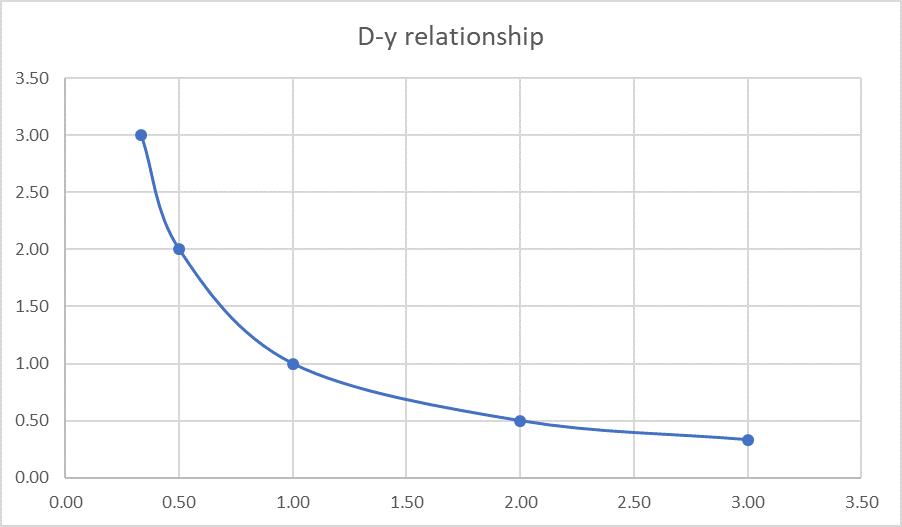
\includegraphics[width=16cm]{img//Newton.PNG}
\caption{牛顿迭代法}
\label{fig:sys.param}
\end{center}
\end{figure}

先根据市场年化率,猜测一个$y_1$,
对曲线上点$(y_1, D_1)$和$(y_0, D_0)$,我们可以求出$Duration = dp/dy$,
逐步调整$y_1$的值,缩小$\Delta y$,
把猜测的值往真实值逼近,
也就是牛顿迭代法。
